\documentclass[graphics]{beamer}

\usepackage{graphicx}
\usepackage{verbatim}
\usepackage{wrapfig}
\useoutertheme{shadow}
%\usecolortheme{orchid}
\usecolortheme{seahorse}
\usepackage{tikzsymbols}
\usepackage{textcomp}
\usepackage{parskip}

% math commands
\newcommand{\be}{\begin{eqnarray}}
\newcommand{\ee}{\end{eqnarray}}
\newcommand{\beq}{\begin{equation}}
\newcommand{\eeq}{\end{equation}}
\def\simless{\mathbin{\lower 3pt\hbox
      {$\rlap{\raise 5pt\hbox{$\char'074$}}\mathchar"7218$}}}
\def\simgreat{\mathbin{\lower 3pt\hbox
      {$\rlap{\raise 5pt\hbox{$\char'076$}}\mathchar"7218$}}} %> or of order

% variables

\def\toonscale{0.45}
\def\mboxy#1{\mbox{\small #1}}


\begin{comment}
\AtBeginSection[]{
  \frame{
    \frametitle{Outline}
    \tableofcontents[currentsection]
  }
}
\end{comment}

\title{Magnetic Helicity
}
\subtitle{}
\author[U. Pen]{\textcolor{green}{Ue-Li Pen}
\\[8mm] 
}
\date{February 4, 2023}


\begin{document}

\frame{
\titlepage
}

%\section*{Introduction}
\section{Magnetic Helicity}

\begin{comment}
  \subsection{Outline}

  \frame{
    \frametitle{Outline}
    \tableofcontents
  }
\end{comment}

  \frame{
    \frametitle{Nature}
\vspace{-0.3in}\center{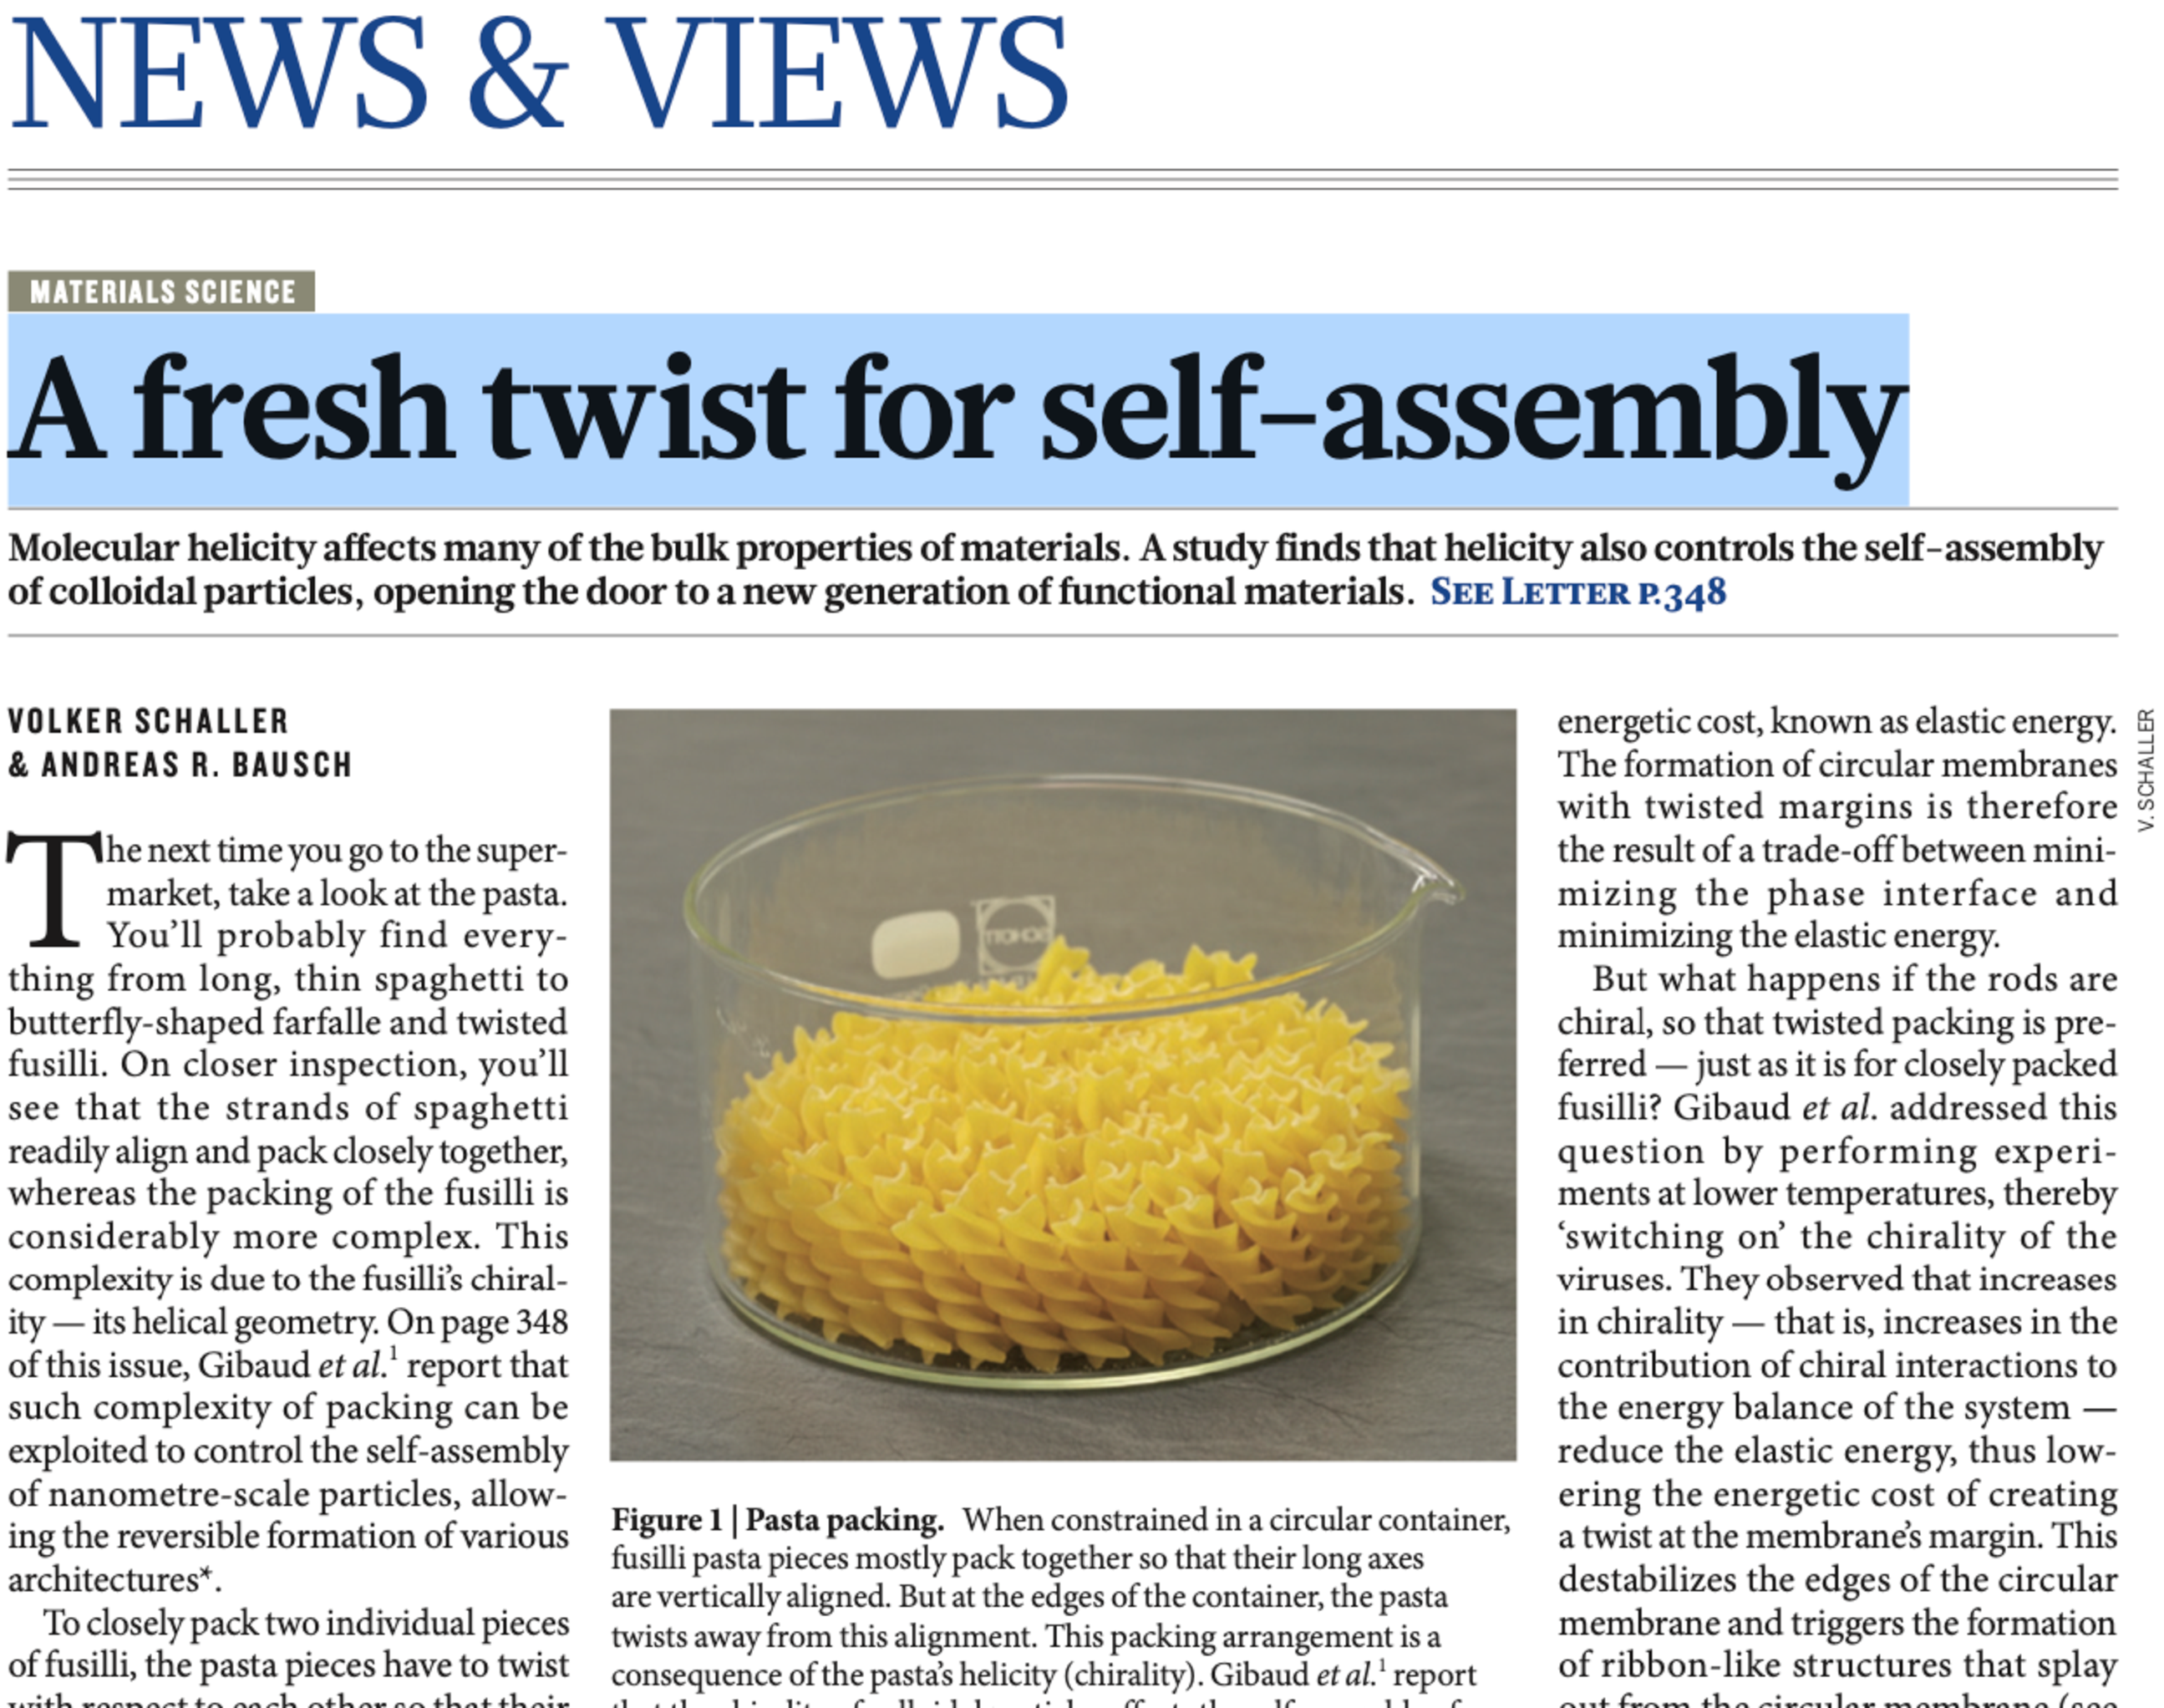
\includegraphics[width=4.0in]{Figures/twist.pdf}}
V Schaller \& A. Bausch 2012, Nature, 481, 268
}
  \frame{
    \frametitle{Pastarimeter}
    %\vspace{-0.3in}
    \center{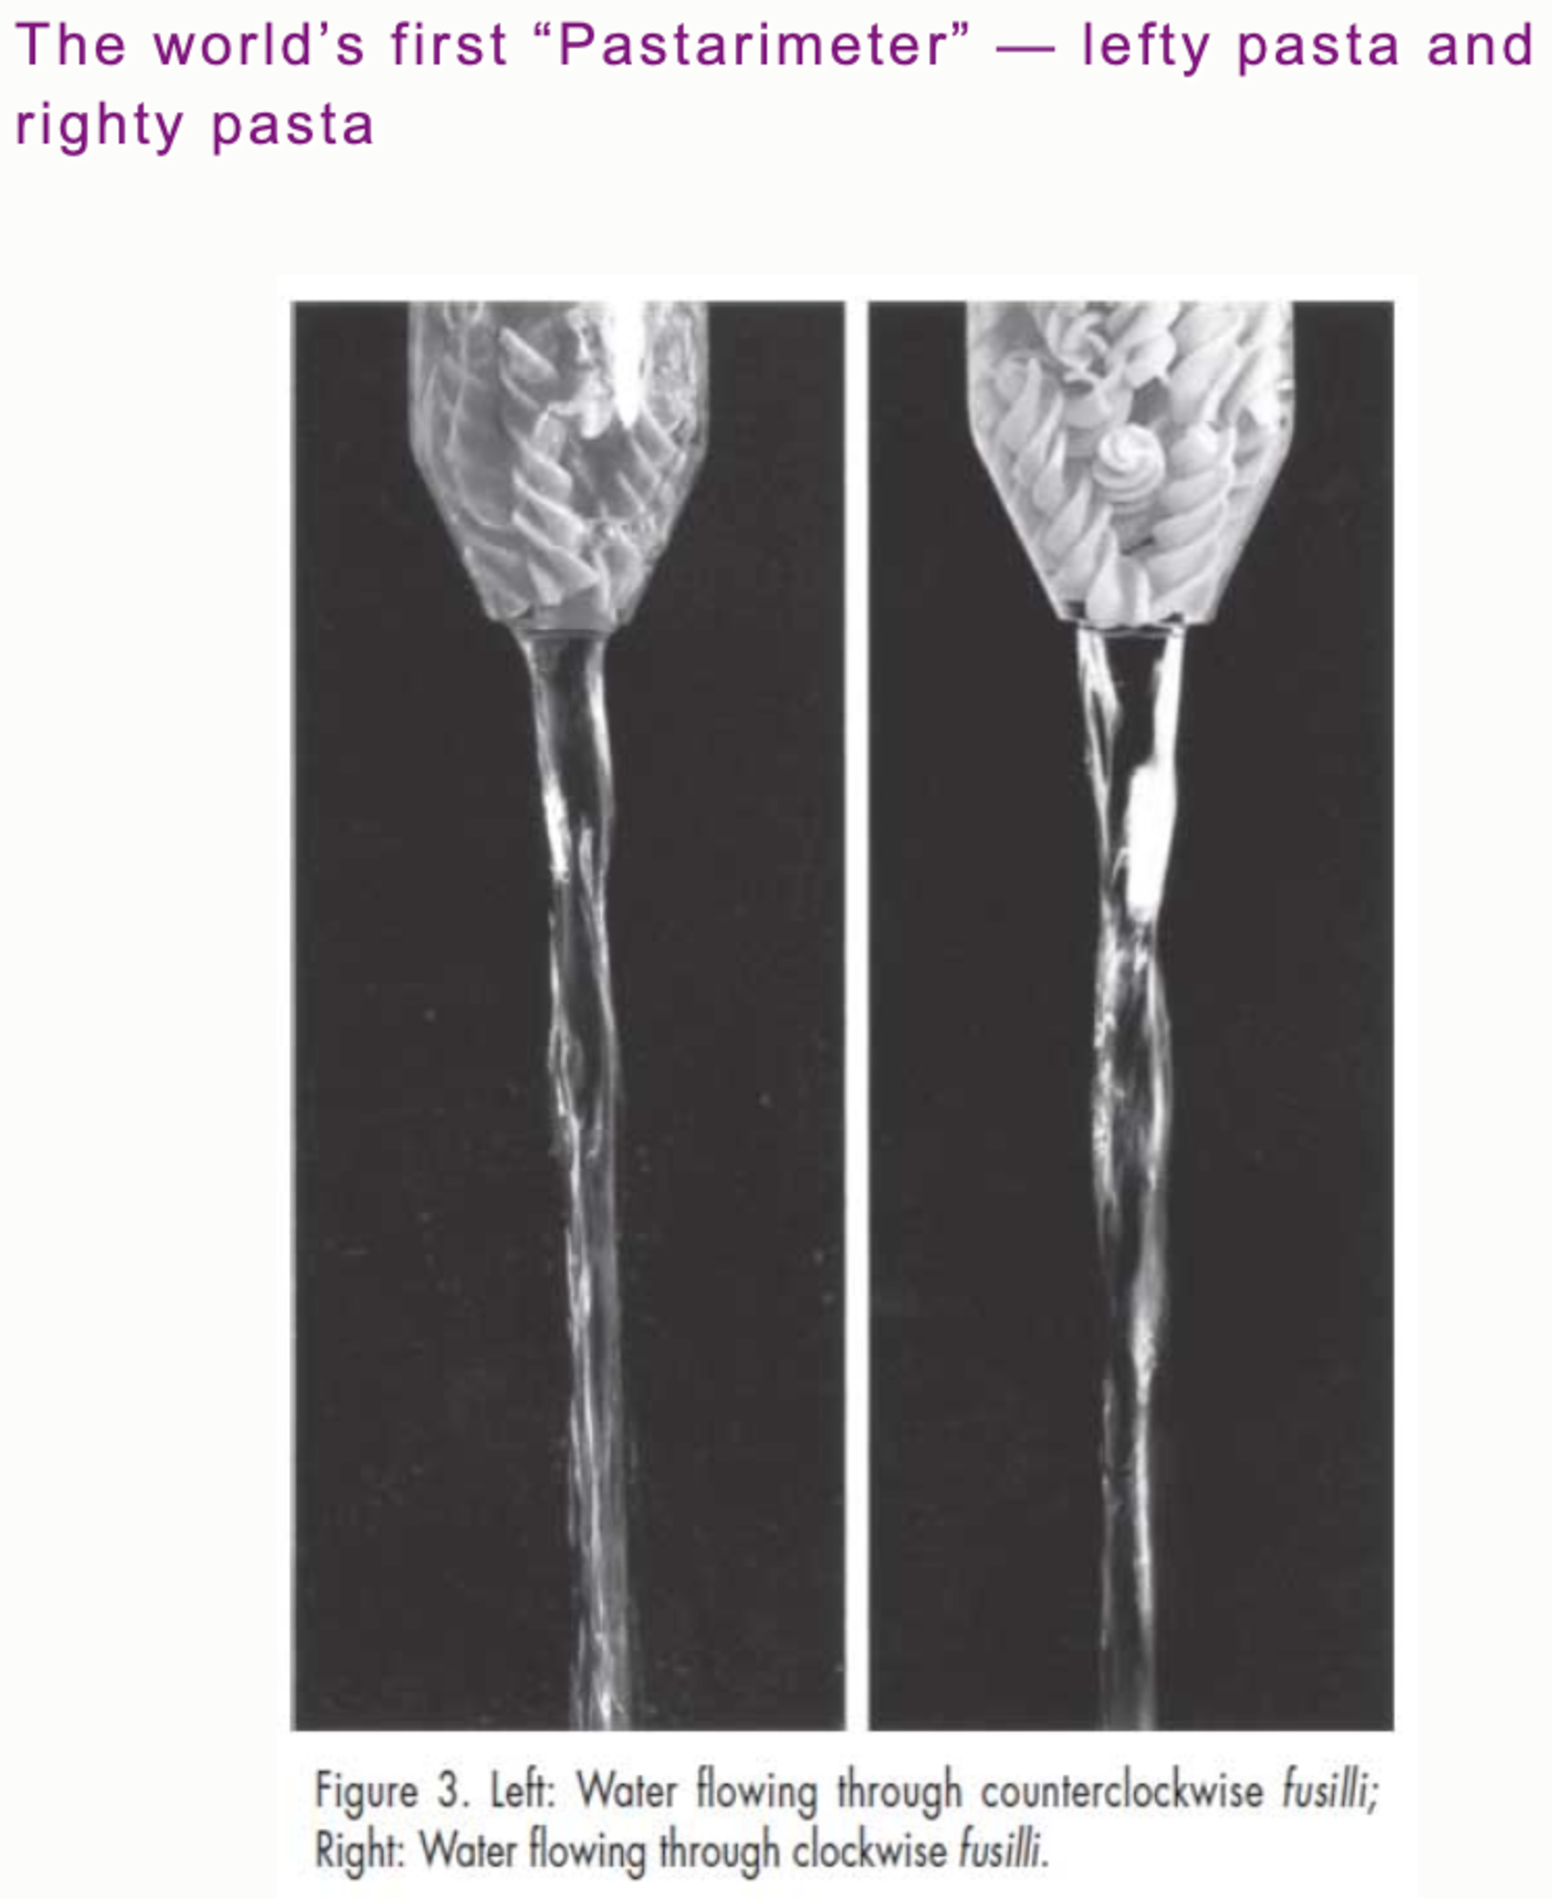
\includegraphics[width=2.5in]{Figures/pastarimeter.pdf}}
{\tiny Saxon et al 2002, J. Chem. Ed, 79, 1214}
}


  \frame{
    \frametitle{Cosmic magnetic Fields}
\begin{itemize}
\item origin and evolution of magnetic fields on many scales still
  open problem
\item earth magnetic field: considered solved, resistive dynamo due to
  rotating, convecting, liquid iron core with solid inner buffer
\item Sun: regular 11 year cycle: challenging to understand due to
  gigayear resistive time scale
\item galaxy: kpc coherent field, similarly challenging with even
  longer time resistive time scale
\item cluster, etc
\item primordial?
\end{itemize}
}


  \frame{
    \frametitle{Earth}
%\vspace{-0.3in}
\center{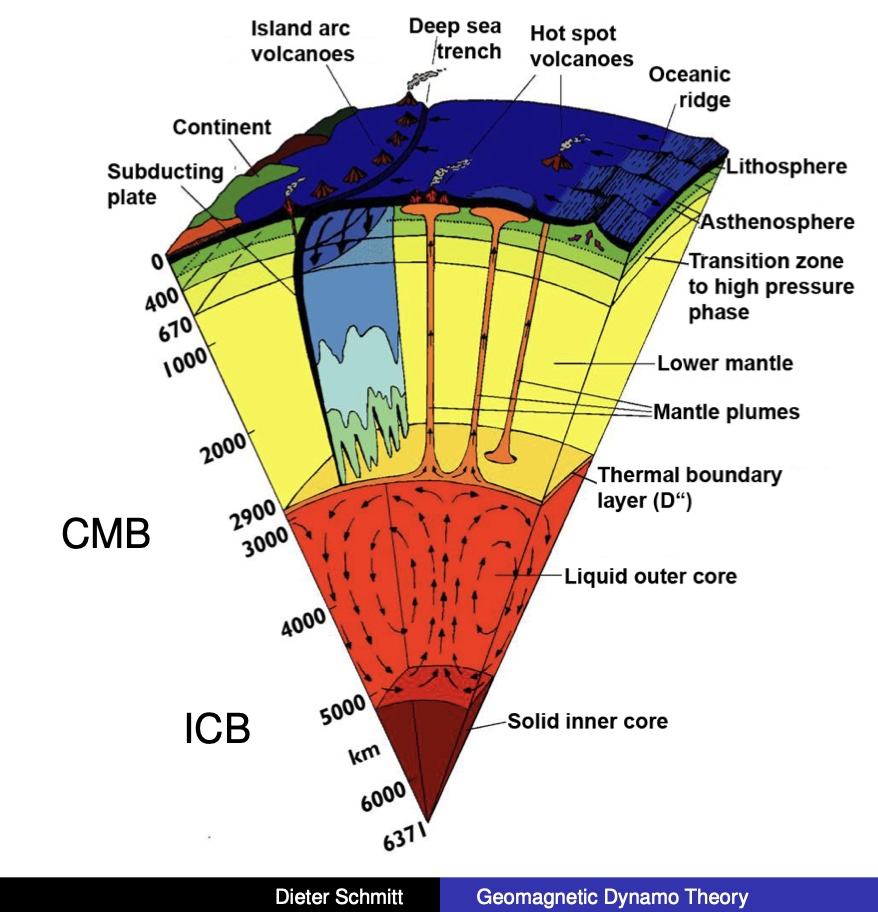
\includegraphics[width=3.0in]{Figures/earth.jpg}}
}

  \frame{
    \frametitle{Core}
%\vspace{-0.3in}
\center{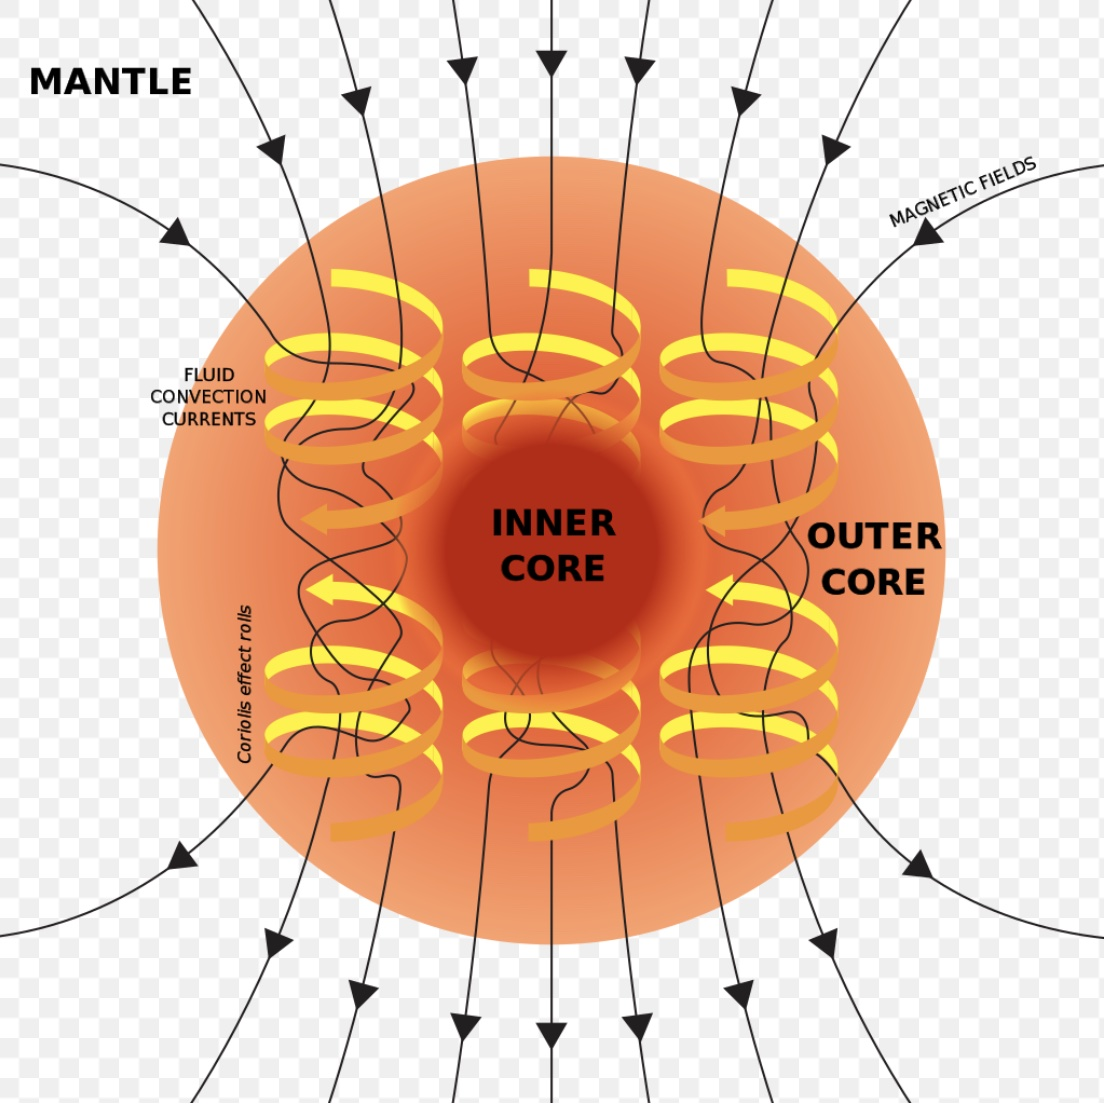
\includegraphics[width=2.5in]{Figures/core.jpg}}

wikipedia: A. Colvin
}


  \frame{
    \frametitle{Sun}
%\vspace{-0.3in}
\center{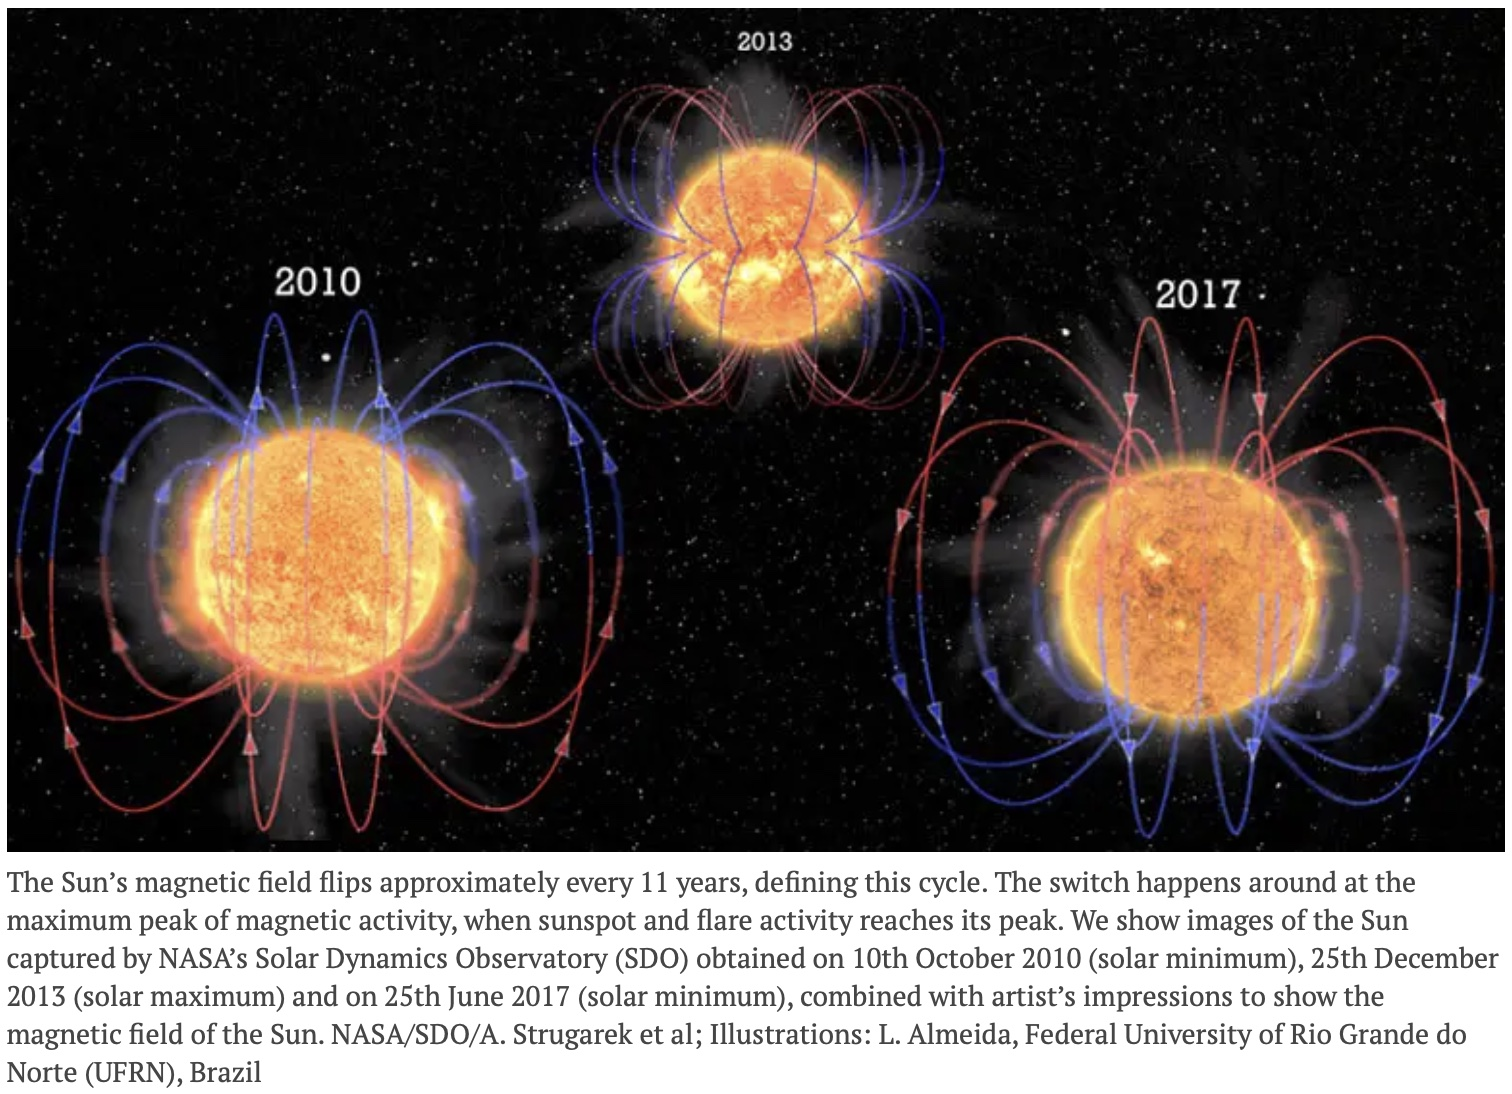
\includegraphics[width=4.2in]{Figures/sunflip.jpg}}
}


  \frame{
    \frametitle{Tachocline}
%\vspace{-0.3in}
\center{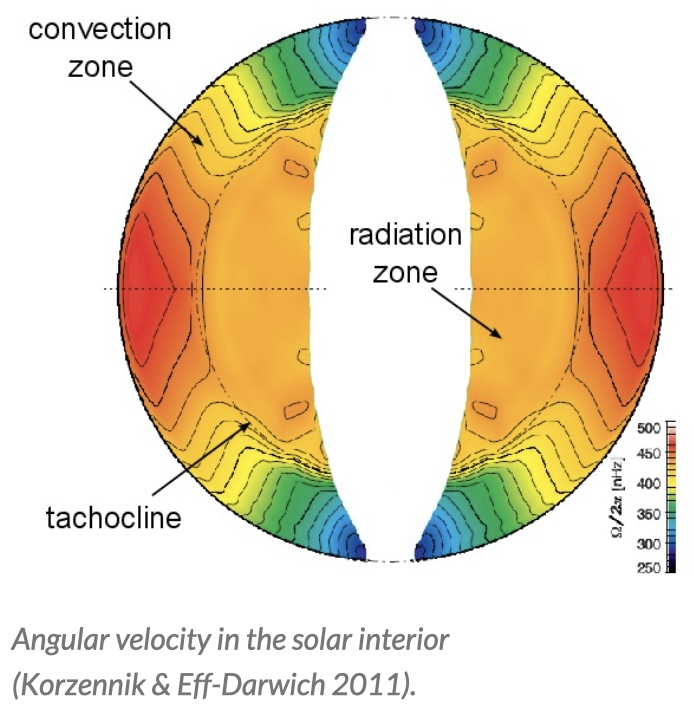
\includegraphics[width=3.0in]{Figures/tachocline.jpg}}
}

  \frame{
    \frametitle{MW}
%\vspace{-0.3in}
\center{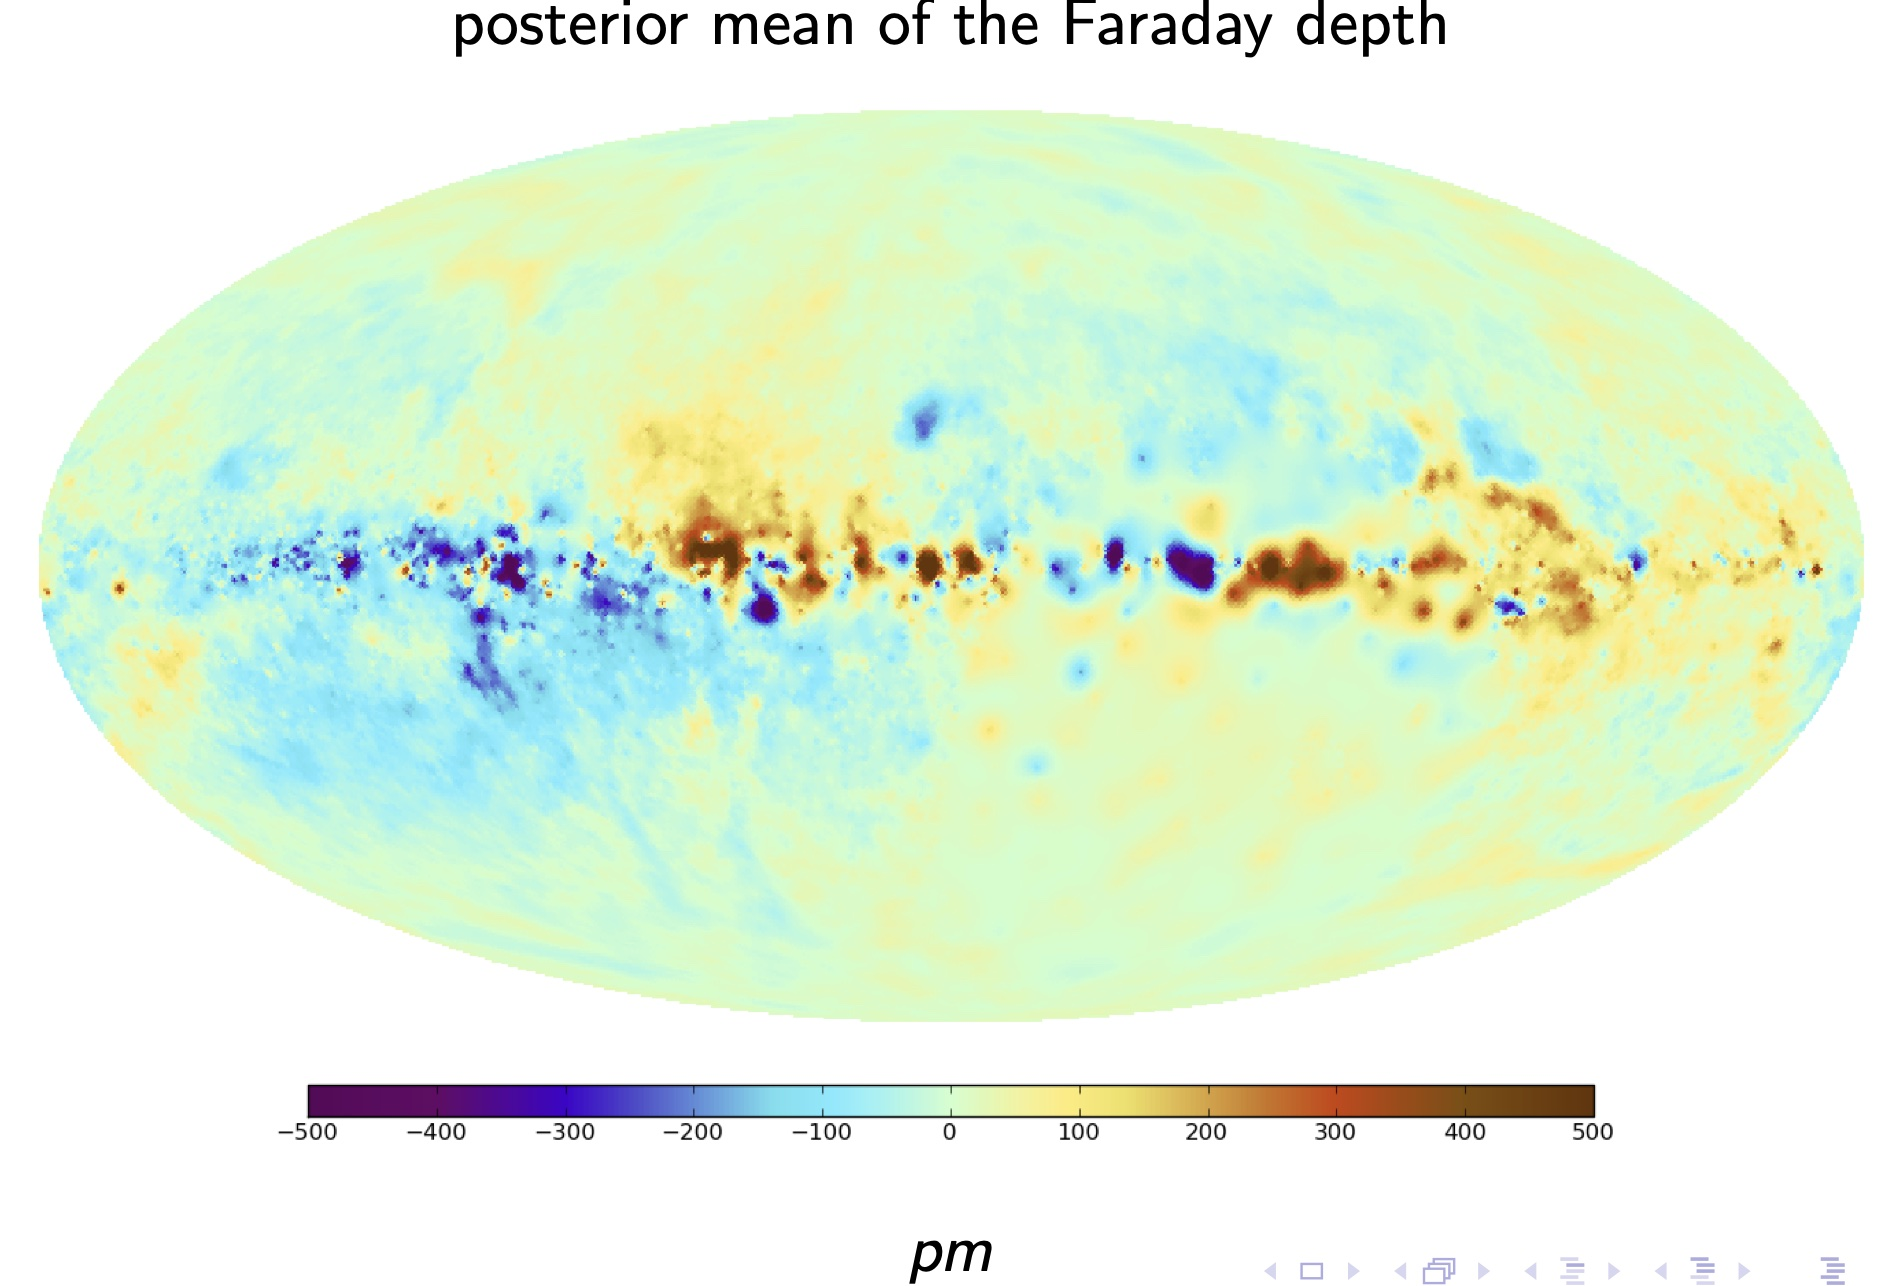
\includegraphics[width=4.0in]{Figures/mw.jpg}}

Niels Oppermann
}

  \frame{
    \frametitle{NGC5775}
%\vspace{-0.3in}
\center{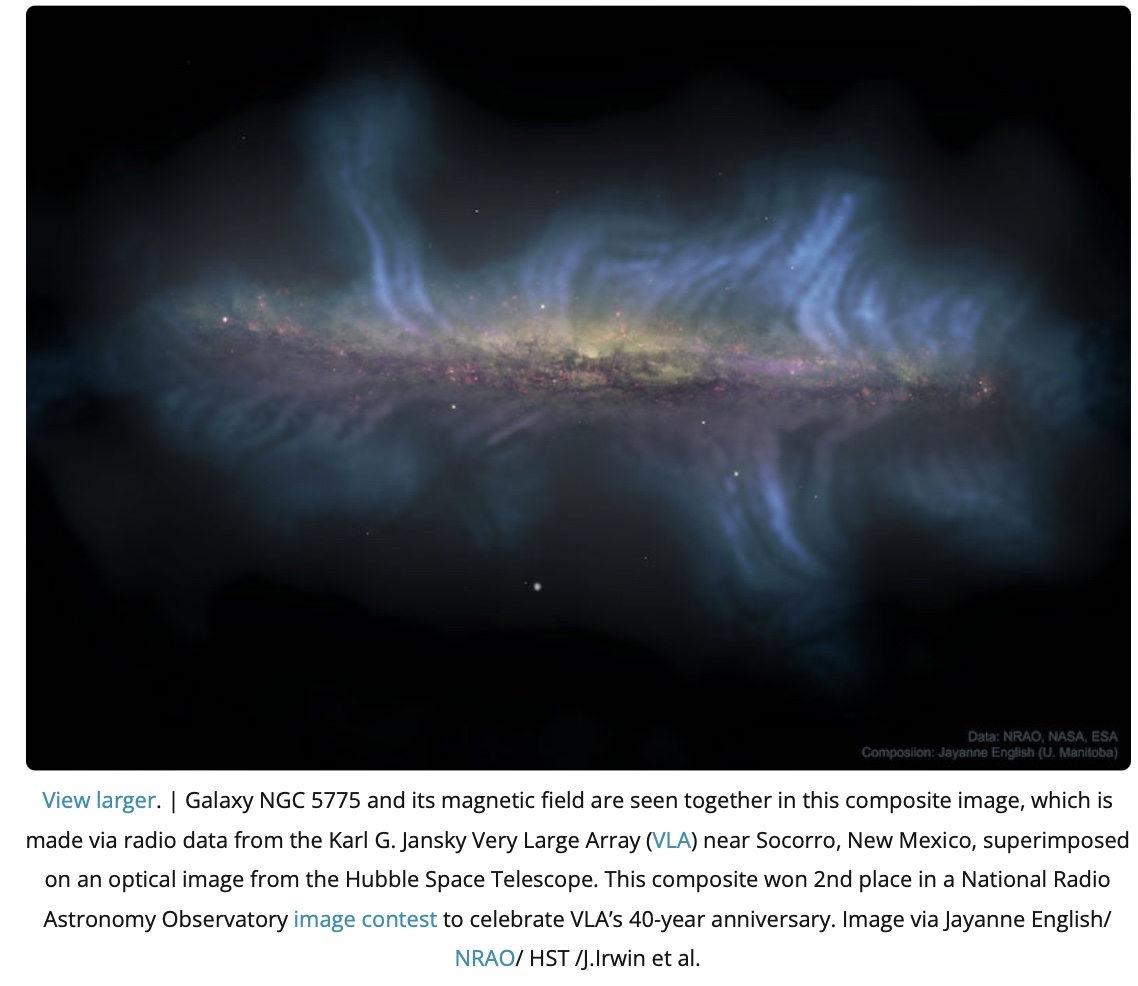
\includegraphics[width=3.5in]{Figures/ngc5775.jpg}}
}




  \frame{
    \frametitle{Helical dynamo?}
\begin{itemize}
\item Magnetic helicity has a key ingredient in many dynamo models
\item $H=\int A\cdot B$: projection of vector potential and magnetic field
\item Helicity leads to inverse turbulent cascade
\item relevant in rotating systems
\item primordial?
\end{itemize}
}


  \frame{
    \frametitle{Helicity from the ground up}
\begin{itemize}
\item any vector $\vec{v}=\nabla \phi+\nabla \times A =
  \nabla\phi+\nabla_L\phi_L+\nabla_R \phi_R$
\item leads to inverse turbulent cascade
\item relevant in rotating systems
\item primordial fields
\end{itemize}
}


  \frame{
    \frametitle{projection operators}
\begin{itemize}
\item curl is a matrix
  $\nabla\times=\left(\begin{array}{ccc}
0 &-\partial_z&\partial_y \\
\partial_z&0&-\partial_x \\
-\partial_y&\partial_x&0
\end{array}\right)$
\item in Fourier space: $\tilde{\nabla}\times=\left(\begin{array}{ccc}
0 &-ik_z&ik_y \\
ik_z&0&-ik_x \\
-ik_y&ik_x&0
\end{array}\right)$
\item factor $=|k|\left(\begin{array}{ccc}
0 &-i\hat{k}_z&i\hat{k}_y \\
i\hat{k}_z&0&-i\hat{k}_x \\
-i\hat{k}_y&i\hat{k}_x&0
\end{array}\right)=|k|\bf{C}$
\item unit curl matrix $\bf{C}$ has three eigenvalues: -1,0,1
  corresponding to left helical, divergence, right helical, and
  eigenvectors $\bf{e}_L,\ \bf{e}_D,\ \bf{e}_R$.
\item it follows that $\tilde{\nabla}_\alpha = |k| \bf{e}_\alpha$ and similarly for $\nabla$
\end{itemize}
}

  \frame{
    \frametitle{potentials}
\begin{itemize}
\item we thus have $\nabla^2 \phi_L=\nabla_L \cdot \vec{v}$ etc
\item NB: divergence is the zero eigenvector, $\nabla_D=\nabla$
\item $B_L=|k|A$,  $B_R=|k|A_R$, and helicity $A\cdot B=\pm|k|A^2$ projects
  the local helicity. 
\end{itemize}
}

  \frame{
    \frametitle{Model system}
\begin{itemize}
\item axionic baryogenesis
\item $\dot{B}=\nabla \times E+g \dot{\theta} \nabla \times B$
\item $\dot{B}_L=-g \dot{\theta} |k| B_L$,\ \ \  $\dot{B}_R=g \dot{\theta} |k| B_R$
\item $B_L=\exp\left( -g \dot{\theta} t) B_L(t=0)$,\ \ \  $B_R=\exp\left( g \dot{\theta} t) B_R(t=0)$
\item always an unstable mode, amplifies $B$ fields of single
  helicity.
\item in practice limited by plasma conductivity (Campanelli++05,
  Ng++16)
\item provides weak helical seed field that is subsequently amplified by
  inverse turbulent cascade
\end{itemize}
}
  \frame{
    \frametitle{Kinematics}
\begin{itemize}
\item helicity requires a 3-D field, not definable for 2-D field
\item need a 3-D observable, projected fields not sufficient
\end{itemize}
}

  \frame{
    \frametitle{Polarization}
\begin{itemize}
\item a vector is a spin-1 field described by one index.  Polarization
  is a spin-2 field with Stokes parameters
$P=\langle E_i E_j\rangle = \left(\begin{array}{cc} I+Q &U+iV \\
                                    U-iV&I-Q \end{array}\right)$
\end{itemize}
}

  \frame{
    \frametitle{Observing in 3-D}
\begin{itemize}
\item Measure polarization as function of frequency
\item RM transform to Faraday depth
\item use Faraday depth (RM) as proxy for distance
\item Opperman maps provide sign
\item convert to helical basis $L,R=Q\pm iU$
\item fraction helical power spectrum $f=\frac{L^2-R^2}{L^2+R^2}=\frac{{\rm Im}Q\bar{U}}{Q^2+U^2}$
\end{itemize}
}



  \frame{
    \frametitle{GBT-IM maps: from Jennifer et al}
%\vspace{-0.3in}
\center{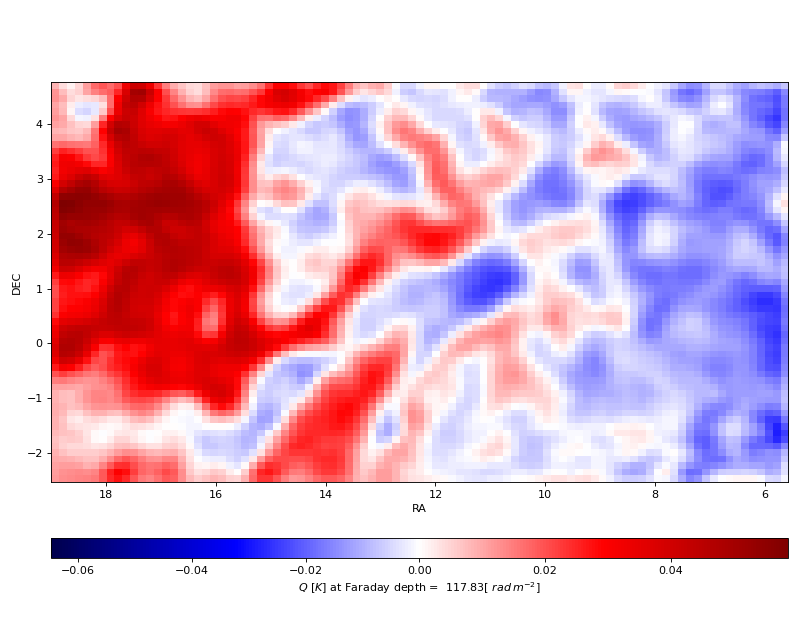
\includegraphics[width=2.0in]{Figures/11hrCom20arcmin_QphiDecRA_plot_map_atSelPhiInd_1000_wPhi_117_83.png}
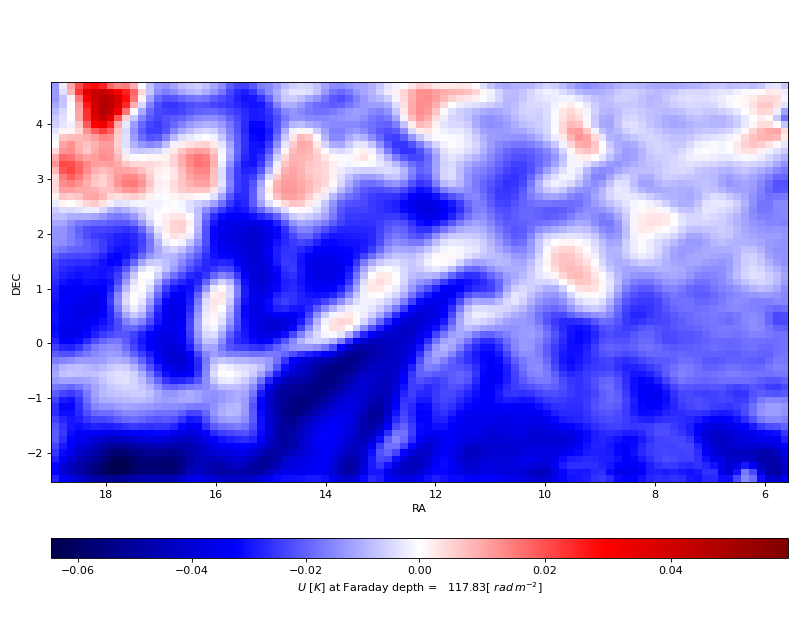
\includegraphics[width=2.0in]{Figures/11hrCom20arcmin_UphiDecRA_plot_map_atSelPhiInd_1000_wPhi_117_83.png}
\\
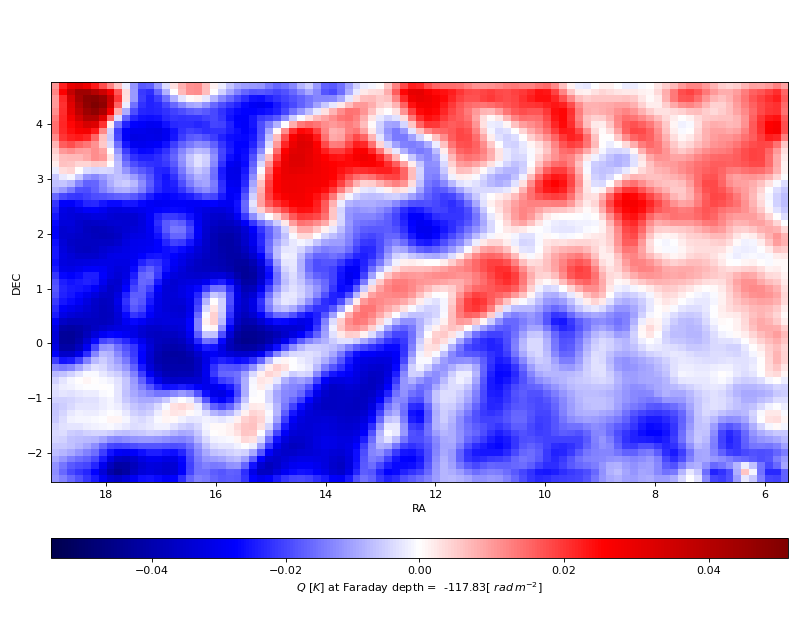
\includegraphics[width=2.0in]{Figures/11hrCom20arcmin_QphiDecRA_plot_map_atSelPhiInd_946_wPhi_-117_83.png}
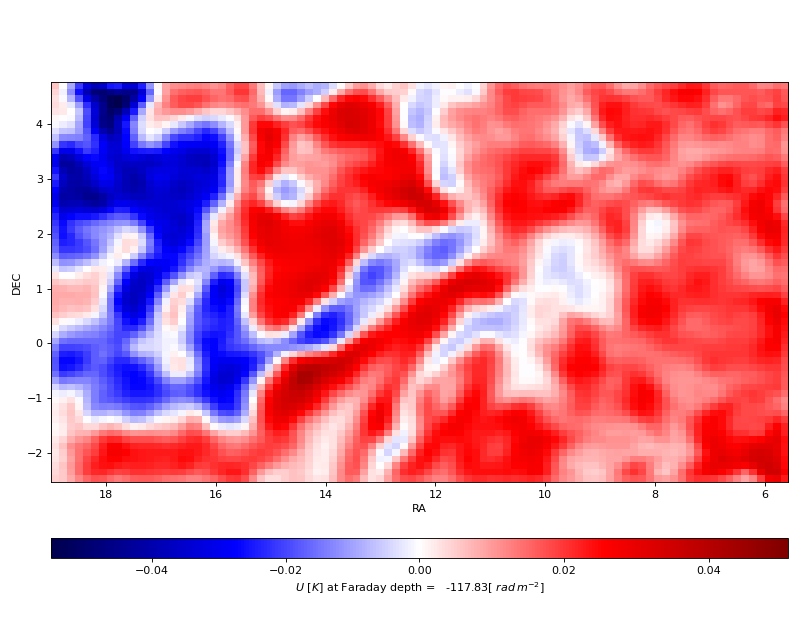
\includegraphics[width=2.0in]{Figures/11hrCom20arcmin_UphiDecRA_plot_map_atSelPhiInd_946_wPhi_-117_83.png}

}
}


\frame{
    \frametitle{Outlook}
\begin{itemize}
\item work in progress for direct measurement of helicity from
  polarized maps: GBT, CHIME, GMIMS
\item history was limited by helicity education in observational measurements
\item direct tests for helical dynamo and primordial helical fields
  (axionic)
\item opportunity for new discovery!
\end{itemize}
}



\end{document}
